%
% This is a borrowed LaTeX template file for lecture notes for CS267,
% Applications of Parallel Computing, UCBerkeley EECS Department.
% Now being used for CMU's 10725 Fall 2012 Optimization course
% taught by Geoff Gordon and Ryan Tibshirani.  When preparing 
% LaTeX notes for this class, please use this template.
%
% To familiarize yourself with this template, the body contains
% some examples of its use.  Look them over.  Then you can
% run LaTeX on this file.  After you have LaTeXed this file then
% you can look over the result either by printing it out with
% dvips or using xdvi. "pdflatex template.tex" should also work.
%

\documentclass[twoside]{article}
\setlength{\oddsidemargin}{0.25 in}
\setlength{\evensidemargin}{-0.25 in}
\setlength{\topmargin}{-0.6 in}
\setlength{\textwidth}{6.5 in}
\setlength{\textheight}{8.5 in}
\setlength{\headsep}{0.75 in}
\setlength{\parindent}{0 in}
\setlength{\parskip}{0.1 in}

\usepackage{url}
\usepackage{graphicx}
\graphicspath{ {images/} }

%
% ADD PACKAGES here:
%

\usepackage{amsmath,amsfonts,graphicx}

%
% The following commands set up the lecnum (lecture number)
% counter and make various numbering schemes work relative
% to the lecture number.
%
\newcounter{lecnum}
\renewcommand{\thepage}{\thelecnum-\arabic{page}}
\renewcommand{\thesection}{\thelecnum.\arabic{section}}
\renewcommand{\theequation}{\thelecnum.\arabic{equation}}
\renewcommand{\thefigure}{\thelecnum.\arabic{figure}}
\renewcommand{\thetable}{\thelecnum.\arabic{table}}

\DeclareMathOperator*{\argmin}{arg\,min}

%
% The following macro is used to generate the header.
%
\newcommand{\lecture}[4]{
   \pagestyle{myheadings}
   \thispagestyle{plain}
   \newpage
   \setcounter{lecnum}{#1}
   \setcounter{page}{1}
   \noindent
   \begin{center}
   \framebox{
      \vbox{\vspace{2mm}
    \hbox to 6.28in { {\bf Technical Presentation
	\hfill } }
       \vspace{4mm}
       \hbox to 6.28in { {\Large \hfill #2  \hfill} }
       \vspace{2mm}
       \hbox to 6.28in { {\it #3 \hfill #4} }
      \vspace{2mm}}
   }
   \end{center}
   \markboth{Technical Presentation #1: #2}{ #1: #2}
}
%
% Convention for citations is authors' initials followed by the year.
% For example, to cite a paper by Leighton and Maggs you would type
% \cite{LM89}, and to cite a paper by Strassen you would type \cite{S69}.
% (To avoid bibliography problems, for now we redefine the \cite command.)
% Also commands that create a suitable format for the reference list.
\renewcommand{\cite}[1]{[#1]}
\def\beginrefs{\begin{list}%
        {[\arabic{equation}]}{\usecounter{equation}
         \setlength{\leftmargin}{2.0truecm}\setlength{\labelsep}{0.4truecm}%
         \setlength{\labelwidth}{1.6truecm}}}
\def\endrefs{\end{list}}
\def\bibentry#1{\item[\hbox{[#1]}]}

%Use this command for a figure; it puts a figure in wherever you want it.
%usage: \fig{NUMBER}{SPACE-IN-INCHES}{CAPTION}
\newcommand{\fig}[3]{
			\vspace{#2}
			\begin{center}
			Figure \thelecnum.#1:~#3
			\end{center}
	}
% Use these for theorems, lemmas, proofs, etc.
\newtheorem{theorem}{Theorem}[lecnum]
\newtheorem{lemma}[theorem]{Lemma}
\newtheorem{proposition}[theorem]{Proposition}
\newtheorem{claim}[theorem]{Claim}
\newtheorem{corollary}[theorem]{Corollary}
\newtheorem{definition}[theorem]{Definition}
\newenvironment{proof}{{\bf Proof:}}{\hfill\rule{2mm}{2mm}}

% **** IF YOU WANT TO DEFINE ADDITIONAL MACROS FOR YOURSELF, PUT THEM HERE:

\newcommand\E{\mathbb{E}}

\begin{document}
%FILL IN THE RIGHT INFO.
%\lecture{**LECTURE-NUMBER**}{**DATE**}{**LECTURER**}{**SCRIBE**}
\lecture{1}{Introduction to Non-Linear Optimization for SLAM}{}{Sally Hui}
%\footnotetext{These notes are partially based on those of Nigel Mansell.}

% **** YOUR NOTES GO HERE:

% Some general latex examples and examples making use of the
% macros follow.  
%**** IN GENERAL, BE BRIEF. LONG SCRIBE NOTES, NO MATTER HOW WELL WRITTEN,
%**** ARE NEVER READ BY ANYBODY.

These notes are informally written and may contain errors. Any such errors are unintentional. 

\section{Motivation}

Understanding non-linear optimization is fundamental to understanding SLAM. After we have features extracted from images, and sensor measurements from LIDAR, IMU, etc., how do we find trajectory of the robot? Through this technical presentation, you will learn how to formulate and solve a simple non-negative least squares optimization (NNLS) problem.

\section{Optimization}

Throughout this talk we are concerned with the following problem:
\begin{equation}
x^* = \argmin_x F(x)
\end{equation}

That is, we seek to find the estimation parameter $x$, within a feasible set, that minimizes the objective function $F(x)$. An objective function is one that maps the parameters onto the set of real numbers. This is the ``cost'' function associated with the problem.

This means that when we want to pose an optimization problem, we will have to define the parameter(s) of the problem and a cost function to minimize.

\section{Problem Definition}

To demonstrate the techniques involved, a toy example will be presented. The problem to be solved is illustrated (only draw 2 poses):
\begin{figure}[h]
      	\centering
      	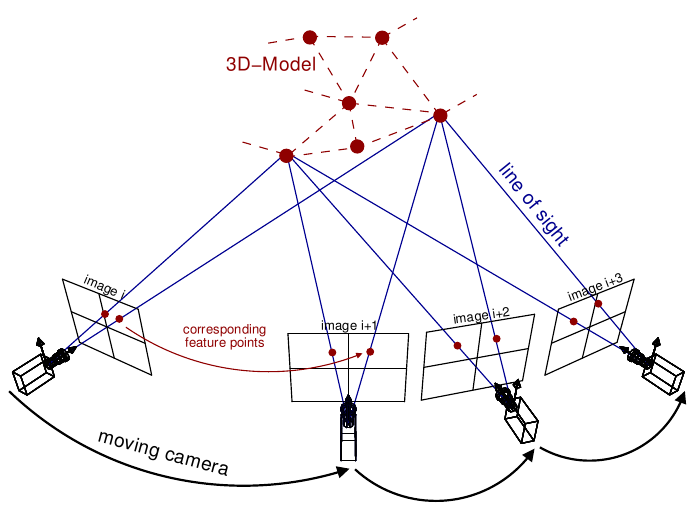
\includegraphics[scale=0.2]{incremental_sfm.png}
      	\caption{http://www.theia-sfm.org/sfm.html}
\end{figure}

Recall that we refer to an object's position and orientation as its \textit{pose}.

A camera moves between two poses. At each pose, the camera can see a common set of $n$ points, with index \textit{1} to \textit{n}. Assume that they have been triangulated (may be explain it in few words) between the two poses, and are denoted in the frame of the first camera as $Z_1^1 \cdots Z_n^1$. Each of their image coordinates, as observed by the second camera, are denoted $z_1^2 \dots z_n^2$ (may be explain what you mean by upper and lower scripts, and lower and upper case Z). Find the transformation $T^{2:1} \in \mathbf{SE(3)}$ (the estimation parameter) that takes points in the frame of the camera's first pose to the frame of the camera's second pose.

Recall that by $\mathbf{SE(3)}$, we refer to the Special Euclidean group representing rigid body transformations. It is a Lie group and a manifold, with a structure $\mathbf{SO(3)} \times \mathbb{R}^3$.

That is, the transformation we seek has the following structure:
\begin{equation}
T =
\begin{pmatrix}
R & t \\
0 & 1\\
\end{pmatrix}
\end{equation}

Here, recall that the group of pure rotations is $R \in \mathbf{SO(3)}$, and the translation is $t \in \mathbb{R}^3$.

To define the cost function we have to define a residual term, or error term. A common one we will use is the reprojection error, which at a point \textit{i} is given by
\begin{equation}
e_i(z_i, x_i) = z^2_i - \pi (T^{2:1} Z_i^1)
\end{equation}

We write $e_i$ as a function of $z_i$ and $x_i$ without $Z_i$, as the 3D points $Z_i$ are assumed to be triangulated from the camera image measurements $z_i$.

$\pi$ is the projection function that takes points from 3D space to the camera's 2D image coordinates. We will use a pinhole model for the camera, and assume no distortion. That is, points in 3D space are mapped to the camera's image by the intrinsic matrix
\begin{equation}
K =
\begin{bmatrix}
f_x & 0 & c_x \\
0 & f_y & c_y\\
0 & 0 & 1 \\
\end{bmatrix}
\end{equation}

and then normalized by dividing by the third coordinate. Recall that $f_x$ and $f_y$ denote the focal length of the camera, which are usually the same, and $c_x$ and $c_y$ denote the center of the camera relative to the origin.

With a slight abuse of notation this gives the projection function $\pi : \mathbb{R}^3 \rightarrow \mathbb{R}^2 $ defined by the equation
\begin{equation}
\pi 
\begin{pmatrix}
\begin{bmatrix}
x \\
y \\
z \\
\end{bmatrix}
\end{pmatrix}
 = 
\begin{bmatrix}
(f_xx + c_xz)/z \\
(f_yy + c_yz)/z \\
\end{bmatrix}.
\end{equation}

We have defined a residual. As the cost function, we will use the sum of squared residuals, which is generally stated as:
\begin{equation}
F(x) = \sum_{i=1}^{n} e_i(z_i, x_i)^T \Omega_i e_i(z_i, x_i),
\end{equation}

where $\Omega$ is the information matrix associated with the problem, and which we'll leave as identity for now. The interpretation of leaving it as identity is that we will trust all measurements equally (we won't weight them unequally).

That is, our optimization problem is:
\begin{equation}
x^* = \argmin_x F(x)
\end{equation}

\section{Gauss-Newton Algorithm}

We will now discuss the most common algorithm used to perform least squares minimization, the basic Gauss-Newton method.

As the cost function is non-linear, we will linearize about a linearization point $\breve{x}$ using a first-order Taylor series expansion:

\begin{equation}
\begin{split}
e_i(\breve{x}_i + \Delta x_i) &= e_i(\breve{x} + \Delta x)\\
&\approx e_i(\breve{x}) + J_i(\Delta x)\\
\end{split}
\end{equation},

where the $J_i$ is the jacobian of the error term.

Plugging this back into the original cost function,
\begin{equation}
\begin{split}
F_i(\breve{x} + \Delta{x}) &= e_i(\breve{x} + \Delta x)^T \Omega_i e_i(\breve{x} + \Delta x) \\
&\approx (e_i(\breve{x}) + J_i \Delta x)^T \Omega_i (e_i(\breve{x}) + J_i \Delta x) \\
&= e_i(\breve{x})^T \Omega_i e_i(\breve{x}) + 2e_i(\breve{x})^T \Omega_i J_i \Delta x + \Delta x^T J_i^T \Omega_i J_i \Delta x \\
&= c_i + 2b_i \Delta x + \Delta x^T H_i \Delta x \\
\end{split}
\end{equation}

So
\begin{equation}
F(\breve{x} + \Delta{x}) = c + 2b^T \Delta x + \Delta x^T H \Delta x 
\end{equation}

Where we define $c_i$, a constant term, as $e_i(\breve{x})^T \Omega_i e_i(\breve{x})$, $b_i$ as $e_i(\breve{x})^T \Omega_i J_i$, and $H_i$ as $J_i^T \Omega_i J_i$.

We can find the parameter values that minimize the cost function by finding the parameter update $\Delta x$ and applying that to the linearization point $\breve{x}$. To do this we find the derivative of the cost function with respect to $\Delta x$, set it to zero, and solve for $\Delta x$. 

The derivative with respect to the parameter update $\Delta x$ is:

\begin{equation}
\frac{\partial F(\breve{x} + \Delta x)}{\partial \Delta x} = 0 + 2b^T + \Delta x^T (H + H^T) 
\end{equation}

According to Schwarz's theorem, a Hessian is symmetric if the following holds, for a function f where the second derivative is with respect to two variables $x$ and $y$:
\begin{equation}
H = \frac{\partial^2 f}{\partial x \partial y} = \frac{\partial^2 f}{\partial y \partial x}
\end{equation}

Since in our case the Hessian is the second derivative of only one parameter x, it automatically satisfies Schwarz's theorem. 

Then, we have:
\begin{equation}
\frac{\partial F(\breve{x} + \Delta x)}{\partial \Delta x} = 0 + 2b^T + 2 \Delta x^T H^T
\end{equation}

Setting it to zero,
\begin{equation}
\begin{split}
0 &=  2b^T + 2 \Delta x^T H^T \\
\Delta x^T H^T &= -b^T \\
H \Delta x &= -b
\end{split}
\end{equation}

This is the update step for the Gauss-Newton algorithm. So to perform the update, we need to find $H$ and $b$, which are $J^TJ$ and $J^Te(\breve{x})$ respectively, if we set $\Omega$ to $I$. How do we find the Jacobian $J$?

\section{Jacobians}

Recall that the Jacobian is of the error term, where we have entries $J_1$ to $J_n$ corresponding to each point observed. This means the Jacobian takes the following structure:

\begin{equation}
J = 
\begin{bmatrix}
J_1 \\
J_2 \\
\vdots \\
J_n \\
\end{bmatrix}
\end{equation}

Where each row corresponds to a measured point.

Recall that a function's Jacobian is simply the matrix of all first-order partial derivatives of the function. Since the only parameter we are varying is the transformation between the two poses of the camera and all other variables are assumed constant, there is simply one partial we need to calculate, 
\begin{equation}
\frac{\partial e}{\partial T^{2:1}}
\end{equation}

Recall that the residual chosen was 
\begin{equation}
\begin{split}
e_i(z_i, x_i) &= z^2_i - \pi (T^{2:1} Z_i^1) \\
\end{split}
\end{equation}

We can use the chain rule:
\begin{equation}
\frac{\partial e}{\partial T^{2:1}} = \frac{\partial e_i}{\partial \pi (T^{2:1} Z_i^1)} \frac{\partial \pi (T^{2:1} Z_i^1)}{\partial T^{2:1} Z_i^1} \frac{\partial T^{2:1} Z_i^1}{\partial T^{2:1}}
\end{equation}

We can now find the expression for each constituent partial derivative. 
The first one is simply 
\begin{equation}
\frac{\partial e_i}{\partial \pi (T^{2:1} Z_i^1)} = -1 
\end{equation}

In the second one, we want to find the partial derivative of the projection function with respect to a 3D point. Recall that the projection function is defined by 
\begin{equation}
\pi 
\begin{pmatrix}
\begin{bmatrix}
x \\
y \\
z \\
\end{bmatrix}
\end{pmatrix}
 = 
\begin{bmatrix}
(f_xx + c_xz)/z \\
(f_yy + c_yz)/z \\
\end{bmatrix}
\end{equation}

We want the Jacobian of this function with respect to the transformed point
\begin{equation}
T^{2:1}Z = 
\begin{bmatrix}
x' \\
y' \\
z' \\
\end{bmatrix}
= Z'
\end{equation}

For ease of notation, let $\pi_1$ represent $(f_xx + c_xz)/z$ and let $\pi_2$ represent $(f_yy + c_yz)/z$.

This means the Jacobian we are finding has the following structure:
\begin{equation}
\frac{\partial \pi (T^{2:1} Z_i^1)}{\partial T^{2:1} Z_i^1} = 
\frac{\partial \pi (Z')}{\partial Z'} = 
\begin{bmatrix}
\frac{\partial \pi_1}{\partial x} & \frac{\partial \pi_1}{\partial y} & \frac{\partial \pi_1}{\partial z} \\
\frac{\partial \pi_2}{\partial x} & \frac{\partial \pi_2}{\partial y} & \frac{\partial \pi_2}{\partial z} \\
\end{bmatrix}
\end{equation}

This gives:
\begin{equation}
\frac{\partial \pi (Z')}{\partial Z'} = 
\begin{bmatrix}
\frac{f_x}{z} & 
0 & 
\frac{-f_x x}{z^2} \\

0 & 
\frac{f_y}{z} & 
\frac{-f_y y}{z^2} \\
\end{bmatrix}
\end{equation}

Finally, we require 
\begin{equation}
\frac{\partial T^{2:1} Z_i^1}{\partial T^{2:1}}
\end{equation}

From [1], we have the following identity:
\begin{equation}
\frac{\partial RZ}{\partial R} = - (RZ)^\times
\end{equation}

Where $R \in \mathbf{SO(3)}$. The proof of that identity is in the appendix of the referenced paper.

We can consider the transformation $T^{2:1}$ as $\mathbf{SO(3)} \times \mathbb{R}^3$. That is,
\begin{equation}
\begin{split}
T(Z) &= 
\begin{pmatrix}
R & t \\
0 & 1\\
\end{pmatrix}
\begin{bmatrix}
x \\ y \\ z \\ 1
\end{bmatrix} \\
&= R
\begin{bmatrix}
x \\ y \\ z
\end{bmatrix}
+ t
\end{split}
\end{equation}

The Jacobian of $T(Z)$ with respect to the variables R and t are therefore
\begin{equation}
\begin{split}
\frac{\partial T^{2:1} Z_i^1}{\partial T^{2:1}} &= 
\begin{bmatrix}
\frac{\partial T(Z)}{\partial R} & \frac{\partial T(Z)}{t}
\end{bmatrix} \\
&= 
\begin{bmatrix}
- (RZ)^\times & I
\end{bmatrix}
\end{split}
\end{equation}

\section{Putting it together}

Now we have the jacobians required, we have all the required parameters to compute an update step of the Gauss-Newton algorithm.

\begin{equation}
\begin{split}
H \Delta x &= -b
\end{split}
\end{equation}

We can compute $H$ by $J^T J$, and $b$ by $J^Te(\breve{x})$.

So, to reiterate, our algorithm is:
\begin{enumerate}
\item Initialize the transformation $T^{2:1}$ 
\item Calculate $H$ by $J^T J$
\item Calculate $b$ by $J^Te$ 
\item Calculate $\Delta x = -H^{-1} b $ 
\item Apply $\Delta x$ to the current estimate of $x$. 
\item Check for some stopping condition (e.g. the norm of $\Delta x$ is smaller than a certain threshold). If the condition is not reached, perform steps 2-6 again. Else, we have found a candidate $T^{2:1}$.
\end{enumerate}
 
\begin{thebibliography}{9}
\bibitem{omg} 
Michael Bloesch, Hannes Sommer, Tristan Laidlow, Michael Burri, Gabriel Nuetzi, Péter Fankhauser, Dario Bellicoso, Christian Gehring, Stefan Leutenegger, Marco Hutter, Roland Siegwart. \textit{A Primer on the Differential Calculus of 3D Orientations.}, \url{https://arxiv.org/pdf/1606.05285.pdf}
\end{thebibliography}

\end{document}




